
\chapter{Tensor Algorithms}

\section{Tensor Contraction Orders}\label{sec:opt_contr}

Throughout the previous chapters, we drew a \emph{lot} of tensor networks. While the theoretical aspect is sufficient for some applications, there are indeed research areas, mostly computational ones such as quantum circuit simulation, where one wants to actually compute the tensor underlying the tensor network.
This is done by the so-called \emph{tensor contractions}.
To see what this means, consider the following 2-tensor diagram, where we contract two tensors $A$ and $B$:
\begin{center}
    \resizebox{0.44\textwidth}{!}{
        \def\Ax{0}
\def\Bx{2}
\def\Cx{7}
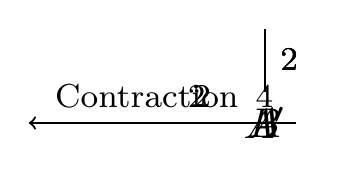
\begin{tikzpicture}[thick, every node/.style={scale=1.5}, tensor/.style={minimum size=0.5cm}]
    \node[tensor] (A) at (\Ax,0) {$A$};
    \node[tensor] (B) at (\Bx,0) {$B$};
    \node[tensor] (Aprime) at (\Cx,0) {$A'$};
    
    \draw (A.north) -- +(0,0.8) node[midway, right] {\footnotesize 2};
    \draw (A.west) -- +(-0.8,0) node[midway, above] {\footnotesize 2};
    \draw (B.north) -- +(0,0.8) node[midway, right] {\footnotesize 2};
    \draw (A.east) -- (B.west) node[midway, above] {\footnotesize 4};
    \draw (Aprime.north) -- +(0,0.8) node[midway, right] {\footnotesize 2};
    \draw (Aprime.west) -- +(-0.8,0) node[midway, above] {\footnotesize 2};

    \draw[->] (\Bx + 1.0, 0) -- (\Cx - 2.0, 0) node[midway, above] {\footnotesize Contraction};
\end{tikzpicture}
    }
\end{center}
Note that we also write the sizes of the respective dimensions, i.e., $A$ is a $2\times 2\times 4$-tensor, while $B$ is a $4 \times 2$-matrix.
Now, the \emph{contraction cost} is defined as the number of FLOPS performed during the contraction; as a convention, this is the number of scalar multiplications.\footnote{This assumes a naive implementation of the operation, i.e., nested loops over the dimensions.}
In our example, the contraction cost is $2 \times 2 \times 4 \times 2 = 32$, i.e., we simply multiply the dimension sizes.

The previous example was rather small.
However, tensor networks in the wild tend to have hundreds of tensors.
Naturally, these also need to be contracted to a single tensor.
Now comes the interesting part: The \emph{order} in which we perform these contraction can have a tremendous impact on the execution time.
To get an intuition for this, consider an extended example of a 3-tensor diagram:
\begin{center}
    \resizebox{0.35\textwidth}{!}{
        \def\Ax{0}
\def\Bx{2}
\def\Cx{4}
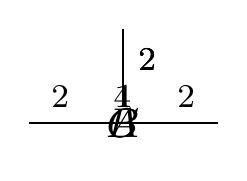
\begin{tikzpicture}[thick, every node/.style={scale=1.5}, tensor/.style={minimum size=0.5cm}]
    \node[tensor] (A) at (\Ax,0) {$A$};
    \node[tensor] (B) at (\Bx,0) {$B$};
    \node[tensor] (C) at (\Cx,0) {$C$};
    
    \draw (A.north) -- +(0,0.8) node[midway, right] {\footnotesize 2};
    \draw (A.west) -- +(-0.8,0) node[midway, above] {\footnotesize 2};
    \draw (B.north) -- +(0,0.8) node[midway, right] {\footnotesize 2};
    \draw (A.east) -- (B.west) node[midway, above] {\footnotesize 4};
    \draw (C.north) -- +(0,0.8) node[midway, right] {\footnotesize 2};
    \draw (C.east) -- +(+0.8,0.0) node[midway, above] {\footnotesize 2};
    \draw (B.east) -- (C.west) node[midway, above] {\footnotesize 1};
\end{tikzpicture}
    }
\end{center}
If we were to contract $A$ with $B$ first (and the resulting tensor with $C$), we would have a cost of $2^2 \times 4\times 2 + 2^3 \times 1 \times 2^2 = 32 + 32 = 64$ multiplications, whereas performing the contraction between $B$ and $C$ at the beginning would result in $2^3 \times 1 \times 2^2 + 2^2 \times 4 \times 2^3 = 32 + 128 = 160$ multiplications in total. Hence, the first order is much better.

It is thus natural to ask: \emph{Can we always find the optimal contraction order?}

\subsection{Algorithms}

We summarize well-known results and frameworks to find good contraction orders.

\subsubsection{Optimal Algorithms}

Indeed, finding the \emph{optimal} contraction order for arbitrary tensor network shapes is pretty hard; better said, NP-hard~\cite{ordering_np_hard}. There is a well-known exact algorithm running in $O(3^n)$-time~\cite{ordering_exact_algo}, where $n$ is the number of tensors in the network. This finds the optimal contraction order with respect to the total contraction cost. If one is interested in minimizing the size of the largest intermediate tensor, i.e., to optimize for the memory used during the execution, this can be done faster in $O(2^n n^3)$-time~\cite{dpconv}. 

The good news is that for some restricted shapes of tensor networks, there are indeed efficient algorithms. A classic example is that dynamic programming solution for the matrix-chain problem~\cite{cormen}, which is just \emph{our} problem, but only for matrices. The naive algorithm runs in $O(n^3)$-time, but can be implemented in $O(n^2)$-time~\cite{mc_yao} (or even in $O(n \log n)$-time~\cite{mc_nlogn_1, mc_nlogn_2}). Another shape for which polynomial-time algorithms exist is that of \emph{tree} tensor networks~\cite{ttn_size, ttn_cost}.

Another prominent way to optimize contraction orders is via the tree decomposition of the \emph{line graph} representation of the tensor network~\cite{markov_shi, dudek_tree_decomp, roman_tree_decomp}. In particular, this results in a contraction order with a maximal intermediate tensor rank equal to the treewidth of the tree decomposition. Loosely speaking, treewidth measures how tree-like a graph is. This does not directly solve our problem since finding the tree decompositions of the smallest treewidth is itself hard~\cite{treewidth_approx}. Two well-known frameworks to find good tree decompositions are \texttt{QuickBB}~\cite{quick_bb} and \texttt{FlowCutter}~\cite{flow_cutter_1, flow_cutter_2}.

\subsubsection{Best-Effort Algorithms}

% TODO: @Thomas, refer to the `einsum` section.
However, once we want to contract \emph{arbitrary} network shapes, the best we can do is to fall back on heuristics or approximations. Two well-known frameworks are \texttt{opt\_einsum}~\cite{opt_einsum} and \texttt{cotengra}~\cite{cotengra}, which aim to optimize the contraction order (also referred to as ``contraction path'') of arbitrary einsums: For tensor networks where the optimal algorithm would be too slow, \texttt{opt\_einsum} applies an ad-hoc greedy algorithm, while \texttt{cotengra} uses hypergraph partitioning~\cite{kahypar}, along with a Bayesian optimization approach, which has been later refined~\cite{jena_tn_cut}. Other algorithms adopted from database query optimization are implemented in \texttt{netzwerk}~\cite{ttn_cost}. Another option is to \emph{learn} the best contraction orders, e.g., using reinforcement learning~\cite{meirom_tn_rl}.

Naturally, the above heuristics do not come with an optimality guarantee. There exists a $(1+\eps)$-approximation $O^*(2^n / \eps)$-time algorithm that minimizes the sum of the intermediate tensor sizes~\cite{dpconv}.

Worth mentioning is the SQL-view of einsum~\cite{einsum_as_sql}: It allows to perform the entire tensor network contraction on any database engine. Indeed, for some einsum classes, running the contractions on state-of-the-art database engines, such as Hyper~\cite{hyper}, can be much faster than using the de-facto \texttt{numpy}-array implementation.
